
\section{Archétype}

\begin{figure}[htbp]
\centering
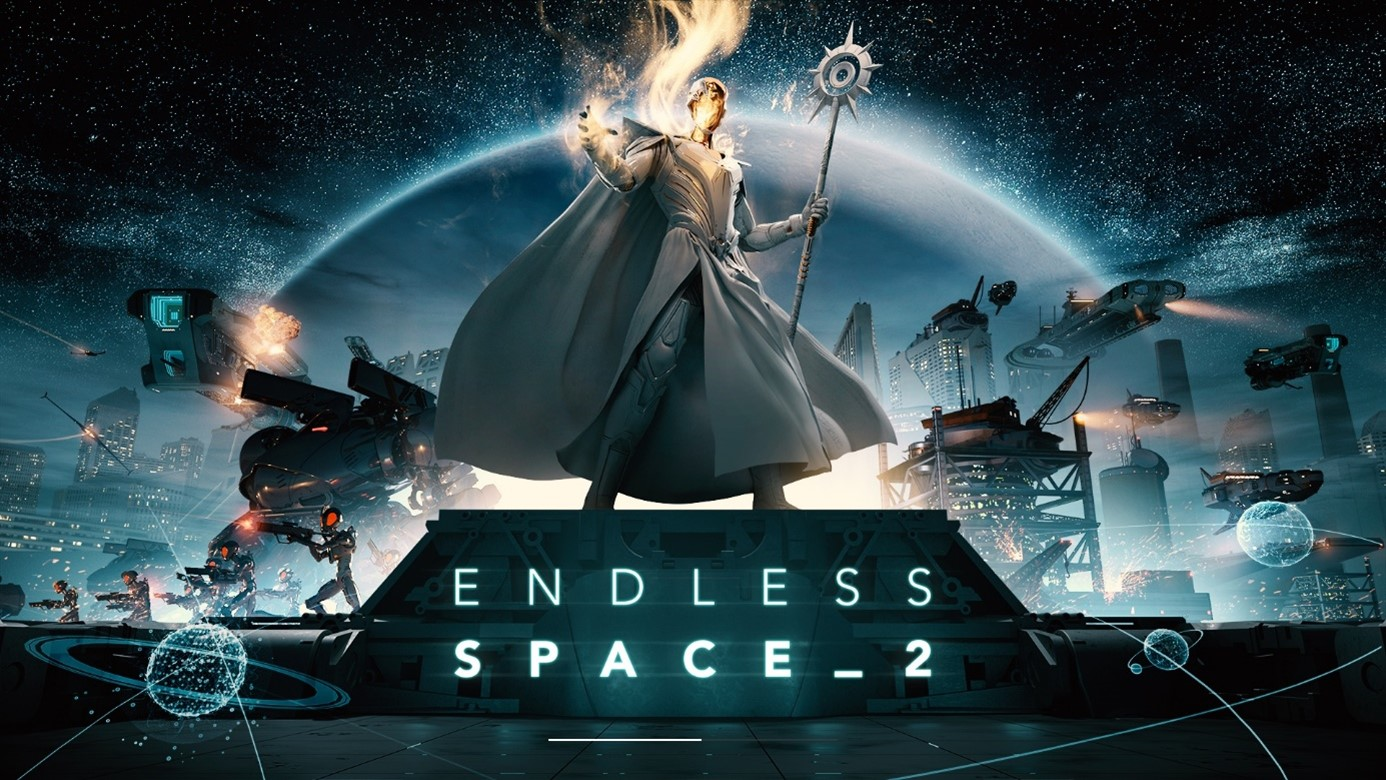
\includegraphics[width=0.9\textwidth]{endless_space_2.jpg}
\caption[Endless Space 2]{\label{figure_simple}Endless Space 2}
\end{figure}

L’objectif de ce projet est de réaliser un jeu de type Endless Space 2. A l’origine, Endless Space 2 est un jeu vidéo de stratégie au tour par tour développé par Amplitude Studios et édité par Sega, dans lequel les joueurs incarnent une civilisation qui devra étendre son influence sur une carte, une galaxie comprenant des systèmes solaires eux-mêmes composés d’une à 4 planètes, générée aléatoirement. Les systèmes solaires font office de « villes » (si on le compare à Civilisation), ils sont reliés entre eux par des voies stellaire, qui eux servent de route. Le joueur peut se déplacer sur la galaxie à l'aide de vaisseaux spatiales militaire ou colonisateur.\\
\begin{figure}[htbp]
\centering
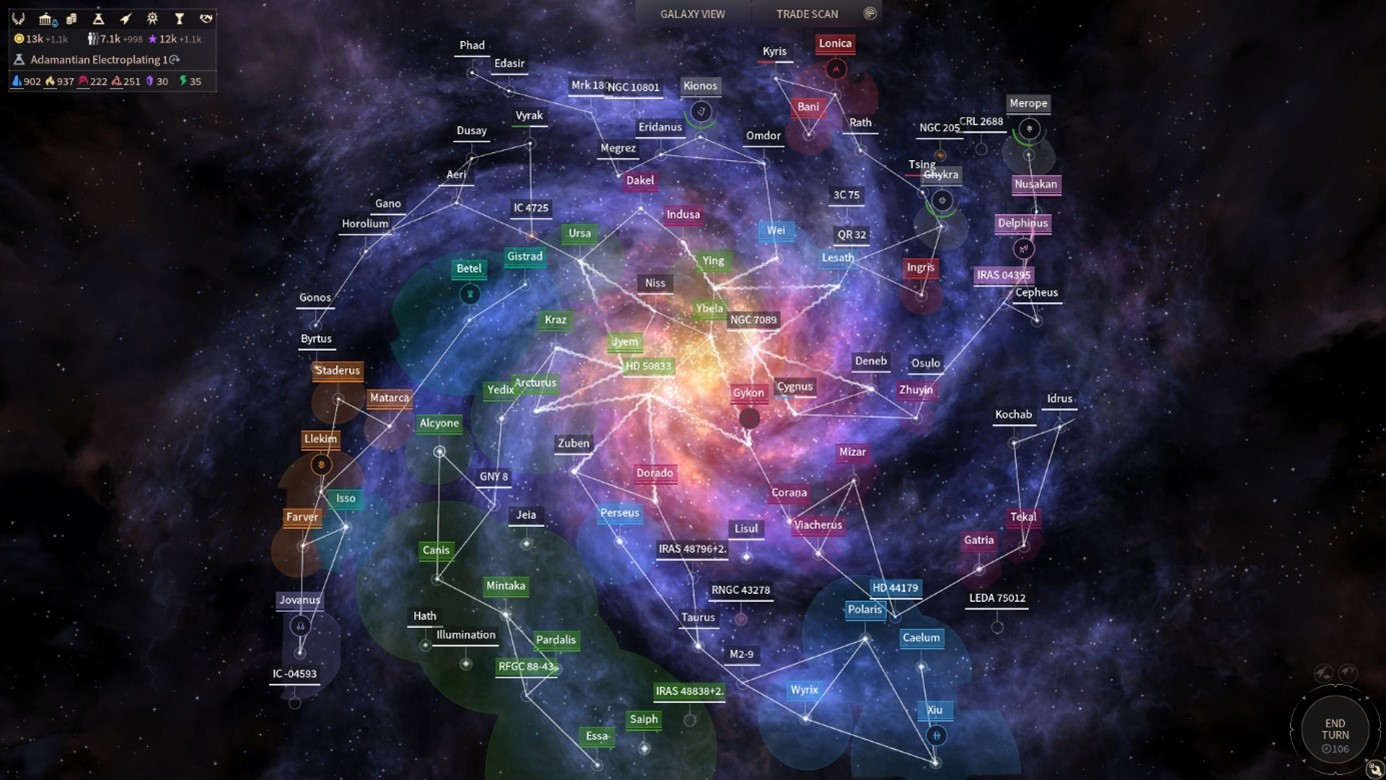
\includegraphics[width=0.9\textwidth]{pics/galaxie.jpg}
\caption[Exemple de galaxie]{\label{figure_simple}Exemple de galaxie}
\end{figure}
\section{Règles du jeu}

En début de partie, vous ne commencez qu’avec une planète colonisée dans l’un des nombreux systèmes stellaire du jeu. Chaque planète produira en quantité plus ou moins importante quatre ressources différentes :\\
\begin{itemize}
\item L’industrie qui servira à la construction de bâtiments et de vaisseaux,
\item La science qui permettra la rechercher de nouvelles technologies et améliorations,
\item La brume comme monnaie unique du jeu pour acheter des bâtiments ou des vaisseaux directement,
\item La nourriture pour augmenter le niveau des planètes.
\end{itemize} 

\begin{figure}[htbp]
\centering
\includegraphics[width=0.9\textwidth]{pics/système_solaire_2.jpg}
\caption[Exemple de système stellaire colonisé par une civilisation]{\label{figure_simple}Exemple de système stellaire colonisé par une civilisation}
\end{figure}

Le but du jeu est d’étendre sa civilisation à l’ensemble de la galaxie et de détruire les autres peuples. Afin de pouvoir rivaliser avec les autres peuples, il vous faudra deux choses : maîtriser l’extension de vos voisins et vous développer plus rapidement qu’eux. Ceci impose de coloniser aussi bien les planètes présentes sur votre système de départ que sur les autres systèmes présents dans la galaxie.\\


\begin{figure}[htbp]
\centering
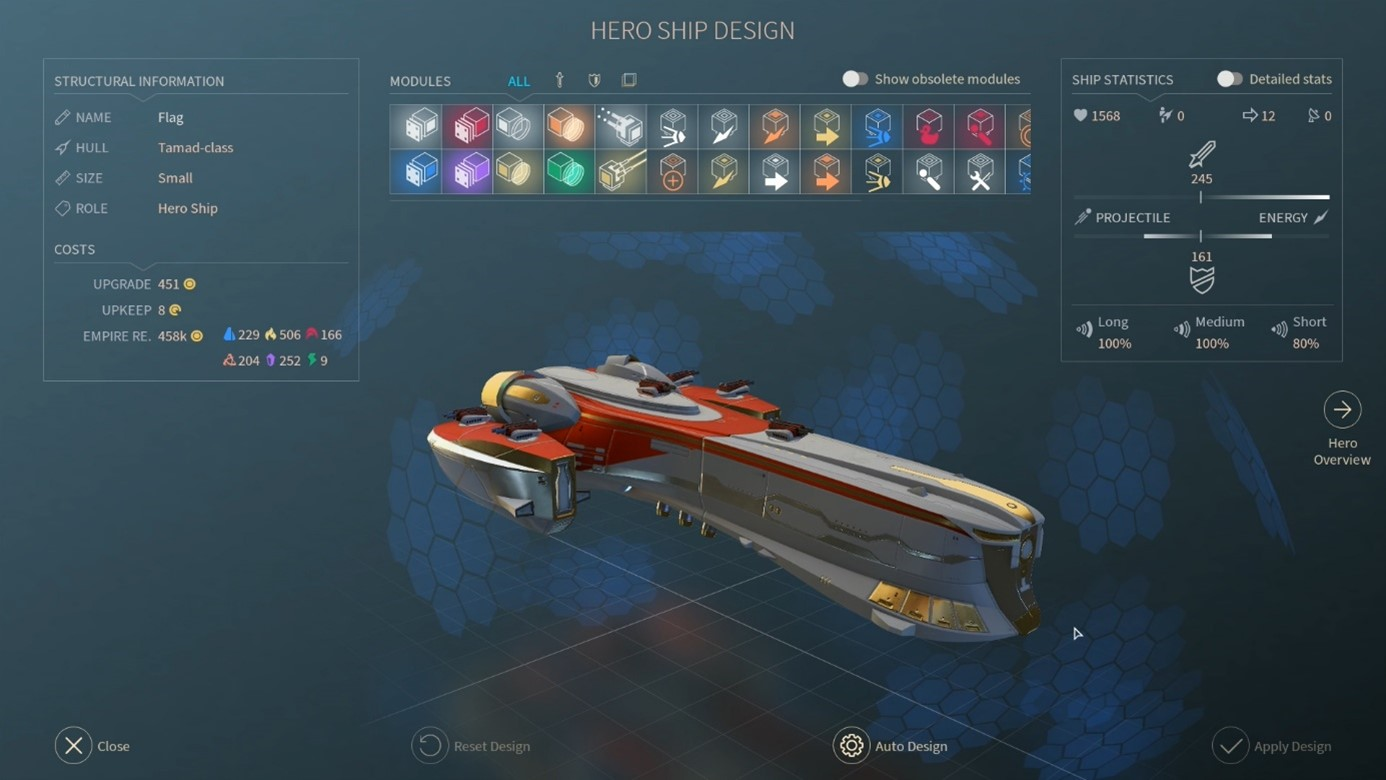
\includegraphics[width=0.9\textwidth]{pics/vaisseau.jpg}
\caption[Exemple de vaisseau]{\label{figure_simple}Exemple de vaisseau}
\end{figure}

Pour gagner une partie d’Endless Space 2, plusieurs solutions s’offrent à vous, allant de celui qui a les plus grosses statistiques à la fin d'un nombre de tour définit, l’éradication pure et simple des autres factions ou arriver à la fin de l'arbre technologique. Côté combat, il n’est possible de se battre qu'uniquement que lorsque votre flotte est en orbite sur un système stellaire, sachant que dès qu’une route est empruntée, il est impossible de faire demi-tour tant que votre flotte n’est pas arrivée à la fin de la voie stellaire. Une fois le combat engagé, soit contre une flotte adverse, soit pour envahir une planète, ceux-ci se dérouleront de manière autonome.



\section{Ressource}

\begin{figure}[htbp]
\centering
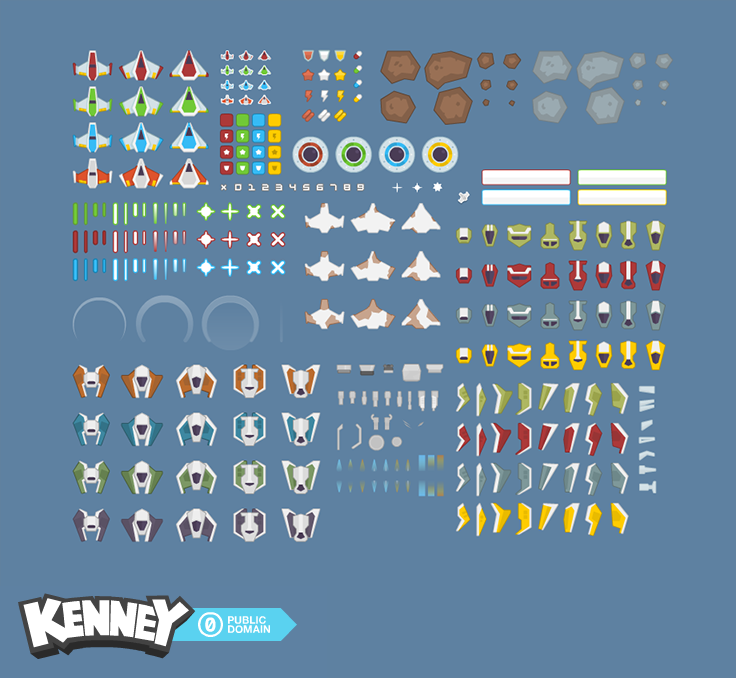
\includegraphics[width=0.9\textwidth]{pics/spaceship_1_preview.png}
\caption[Texture pour les vaisseaux]{\label{figure_simple}Texture pour les vaisseaux}
\end{figure}

\begin{figure}[htbp]
\centering
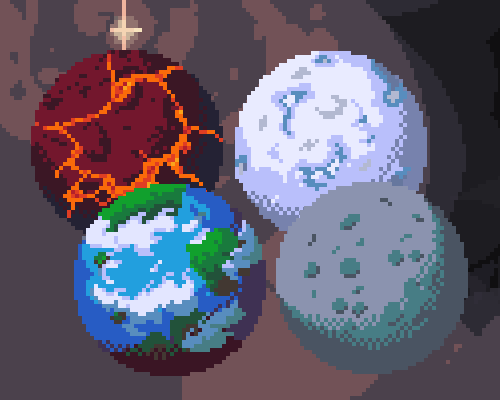
\includegraphics[width=0.9\textwidth]{pics/planets.png}
\caption[Texture pour les planètes]{\label{figure_simple}Texture pour les planètes}
\end{figure}